%Tex root = ProbabilitàEStatistica.tex

\chapter{Distribuzioni di frequenze}
La statistica riguarda i metodi scientifici per raccogliere, ordinare, riassumere e presentare i dati, per trarre valide conclusioni ed eventualmente prendere ragionevoli decisioni sulla base di tale analisi.

\Definizione{variabili alleatorie}{
    Le variabili oggetto di osservazione statistica si classificano in due tipologie:
    \begin{itemize}[label=$\triangleright$]
    \item \textbf{varibili numeriche}: assume solo valori numerici ($\mathrm{N = 0, 1, \dots}$)
        \begin{itemize}[label=$\diamond$]
        \item discrete: insieme dei valori che può assumere è finito o numerabile
        \smallskip
        \item continue: insieme dei valori che può assumere è l'insieme dei numeri reali $\mathbb{R}$ o un intervallo $\mathrm{I \subset \mathbb{R}}$ ($\mathrm{H \in \mathbb{R}}$)
    \end{itemize}
    \medskip
    \item \textbf{variabili categoriche}: $\mathrm{C = marrone, blue, verde, \dots}$
    \end{itemize}
}

I dati che non sono stati ancora ordinati numericamente si dicono \textbf{grezzi}.

Una \textbf{serie} è un ordinamento di dati grezzi in ordine crescente/decrescente.

La differenza tra il più grande e il più piccolo si dice \textbf{campo di variazione}.

\section{Distribuzine di frequenze: classi}
Per studiare i dati a disposizione occorre costruire una \textcolor{viola}{\textbf{distribuzione di frequenze}}: una tabella dove in una colonna si mettono i valori assunti dalla variabile e in un'altra il numero delle volte che tali valori vengono assunti (frequenze).

\esempio{istrogramma}{
    Consideriamo la varibile P peso di un gruppo di 100 studenti.

    \medskip
    \centering
    \begin{tabular}{|c|c|}
    \hline
    \textbf{Peso in kg} & \textbf{Numero di studenti}\\
    \hline
    64 < P $\le$ 66 & 5\\
    \hline
    66 < P $\le$ 68 & 18\\
    \hline
    68 < P $\le$ 70 & 42\\
    \hline
    70 < P $\le$ 72 & 42\\
    \hline
    72 < P $\le$ 74 & 8\\
    \hline
    \textcolor{red}{\textbf{Totale}} & \textcolor{red}{\textbf{100}}\\
    \hline
    \end{tabular}
}

Possiamo definire:
\begin{itemize}[label=$\triangleright$]
    \item \textbf{ampiezza} della classe: differenza tra il valore massimo e il valore minimo
    \item \textbf{valore centrale} della classe: semisomma degli estremi
\end{itemize}

\medskip
Per rappresentare le distribuzioni di frequenze si utilizzano:
\begin{itemize}[label=$\diamond$]
    \item \textbf{istogrammi}: variabili numeriche
    \smallskip
    \item \textbf{diagrammi a barre}: variabili categoriche
\end{itemize}

\subsection{Istogramma}
Un \textcolor{viola}{\textbf{istogramma}} consiste in un \hl{insieme di rettangoli adiacenti aventi base sull'asse x} con:
\begin{itemize}
    \item \textbf{punto medio} nel valore centrale della classe
    \smallskip
    \item \textbf{altezza} proporzionale alla frequenza della classe
    \smallskip
    \item \textbf{area} pari alla frequenza relativa/percentuale della classe
\end{itemize}

In questo modo se si sommano le aree di tutti i rettangoli ottenuti, si ottiene un valore fisso:
\begin{itemize}[label=$\diamond$]
    \item 1: frequenze relative
    \item 100: frequenze percentuali
\end{itemize}

\esempio{diagramma a barre}{
    Si consideri la seguente distribuzione di frequenze:

    \smallskip
    \begin{center}
    \begin{tabular}{|c|c|}
        \hline
        \textbf{Distrubuzione} & \textbf{Frequenze}\\
        \hline
        110 < D $\le$ 130 & 20\\
        130 < D $\le$ 150 & 40\\
        150 < D $\le$ 170 & 60\\
        170 < D $\le$ 210 & 80\\
        \hline
        \textcolor{red}{\textbf{Totale}} & \textcolor{red}{\textbf{200}}\\
        \hline
    \end{tabular}
    \end{center}

    \medskip
    Riferendoci alla tabella in questione vogliamo determinare la frequenza percentuale e costruire il relativo istrogramma.

    \smallskip
    \begin{center}
    \begin{tabular}{|c|c|c|}
        \hline
        \textbf{Distrubuzione} & \textbf{Frequenze} & \textbf{Frequenze $\%$}\\
        \hline
        110 < D $\le$ 130 & 20 & 10$\%$\\
        130 < D $\le$ 150 & 40 & 20$\%$\\
        150 < D $\le$ 170 & 60 & 30$\%$\\
        170 < D $\le$ 210 & 80 & 40$\%$\\
        \hline
        \textcolor{red}{\textbf{Totale}} & \textcolor{red}{\textbf{200}} & \textcolor{red}{\textbf{100$\%$}}\\
        \hline
    \end{tabular}
    \end{center}

    \smallskip
    Riportiamo sull'asse x gli estremi delle classi.

    Ricordando che l'area di ogni rettangolo deve dare le frequenze percentuali, si ha:
    \begin{itemize}[label=$\triangleright$]
    \item \textbf{altezza prima classe}:
    \begin{equation*}
        \frac{10}{(130-150)} = \boldsymbol{0.5}
    \end{equation*}
    \item \textbf{altezza seconda classe}:
    \begin{equation*}
        \frac{20}{(150-130)} = \boldsymbol{1.0}
    \end{equation*}
    \item \textbf{altezza terza classe}:
    \begin{equation*}
        \frac{30}{(170-150)} = \boldsymbol{1.5}
    \end{equation*}
    \item \textbf{altezza quarta classe}:
    \begin{equation*}
        \frac{40}{(210-170)} = \boldsymbol{1.0}
    \end{equation*}
    \end{itemize}

    \begin{figure}[H]
    \centering
    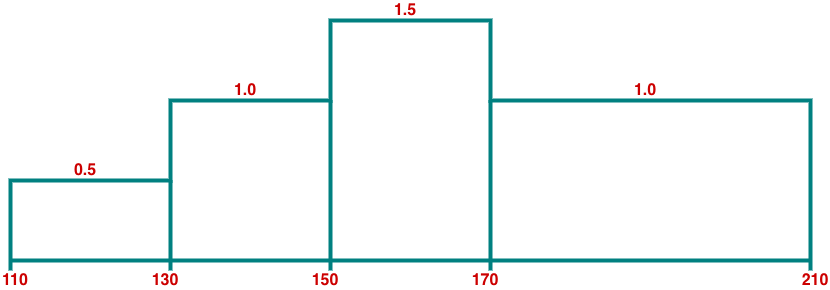
\includegraphics[width=0.6\textwidth]{images/istogramma.png}
    \caption{istogramma}
    \end{figure}
}

\subsection{Diagramma a barre}
I \textcolor{viola}{\textbf{diagramma a barre}} sono dei \hl{rettangoli, non allineati, in cui l'altezza rappresenta la frequenza relativa/percentuale di quella classe}.\\[0.2ex]
Sull'asse x si riportano i tipi, in un oridine deciso dall'osservatore stesso.

\esempio{}{
    Consideriamo le frequenze dei colori degli occhi delle persone:

    \smallskip
    \begin{center}
    \begin{tabular}{|c|c|c|}
        \hline
        \textbf{Colore occhi} & \textbf{Frequenze} & \textbf{Frequenze $\%$}\\
        \hline
        Marrone & 150 & 50$\%$\\
        Blu & 90 & 30$\%$\\
        Verde & 30 & 10$\%$\\
        Altro & 30 & 10$\%$\\
        \hline
        \textcolor{red}{\textbf{Totale}} & \textcolor{red}{\textbf{300}} & \textcolor{red}{\textbf{100$\%$}}\\
        \hline
    \end{tabular}
    \end{center}

    \begin{figure}[H]
    \centering
    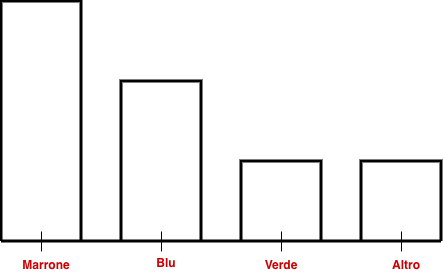
\includegraphics[width=0.6\textwidth]{images/diagramma-barre.png}
    \caption{diagramma a barre}
    \end{figure}
}


\section{Frequenze cumulate e loro rappresentazione}
La \textcolor{viola}{\textbf{frequenza cumulata}} (variabili numeriche) è la \hl{somma di tutte le frequenza inferiori o uguali al confine} di una fissata classe.\\[0.2ex]
Per questo motivo le classi vengono prese aperte a sinistra e chiuse a destra.

Il grafico delle freuqenze cumulata è detto \textbf{ogiva}.

\esempio{calcolo delle frequenze cumulate}{
    Consideriamo le seguenti distibuzioni di frequenza:

    \smallskip
    \begin{center}
    \begin{tabular}{|c|c|}
        \hline
        \textbf{Distrubuzione} & \textbf{Frequenze}\\
        \hline
        110 < D $\le$ 130 & 20\\
        130 < D $\le$ 150 & 40\\
        150 < D $\le$ 170 & 60\\
        170 < D $\le$ 210 & 80\\
        \hline
        \textcolor{red}{\textbf{Totale}} & \textcolor{red}{\textbf{200}}\\
        \hline
    \end{tabular}
    \end{center}

    \medskip
    Riferendoci alla tabella in questione vogliamo determinare la frequenza percentuale cumulata e costruire il relativo grafico.

    \smallskip
    \begin{center}
    \begin{tabular}{|c|c|c|c|}
        \hline
        \textbf{Distrubuzione} & \textbf{Frequenze} & \textbf{Frequenze $\%$} & \textbf{Frequenze cumulate $\%$}\\
        \hline
        110 < D $\le$ 130 & 20 & 10$\%$ & 10$\%$\\
        130 < D $\le$ 150 & 40 & 20$\%$ & 30$\%$\\
        150 < D $\le$ 170 & 60 & 30$\%$ & 60$\%$\\
        170 < D $\le$ 210 & 80 & 40$\%$ & 100$\%$\\
        \hline
        \textcolor{red}{\textbf{Totale}} & \textcolor{red}{\textbf{200}} & \textcolor{red}{\textbf{100$\%$}} & \\
        \hline
    \end{tabular}
    \end{center}

    \begin{figure}[H]
    \centering
    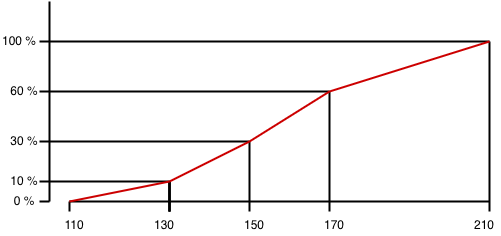
\includegraphics[width=0.6\textwidth]{images/ogiva.png}
    \caption{grafico a ogiva}
    \end{figure}
}